%!TEX root = ../paper.tex
\chapter{程序实现}
	\section{GNU Radio框图}
		\par 按照图\ref{fig:gnuradio_dvbt_tx}在GNU Radio中搭建DVB-T发射端,图\ref{fig:gnuradio_dvbt_rx}在GNU Radio中搭建DVB-T接收端。
		\par 在右侧的模块中选择相应模块,使用Ctrl+f快捷键能更快的找到相应的模块。
		\begin{figure}[htb]
			\centering
			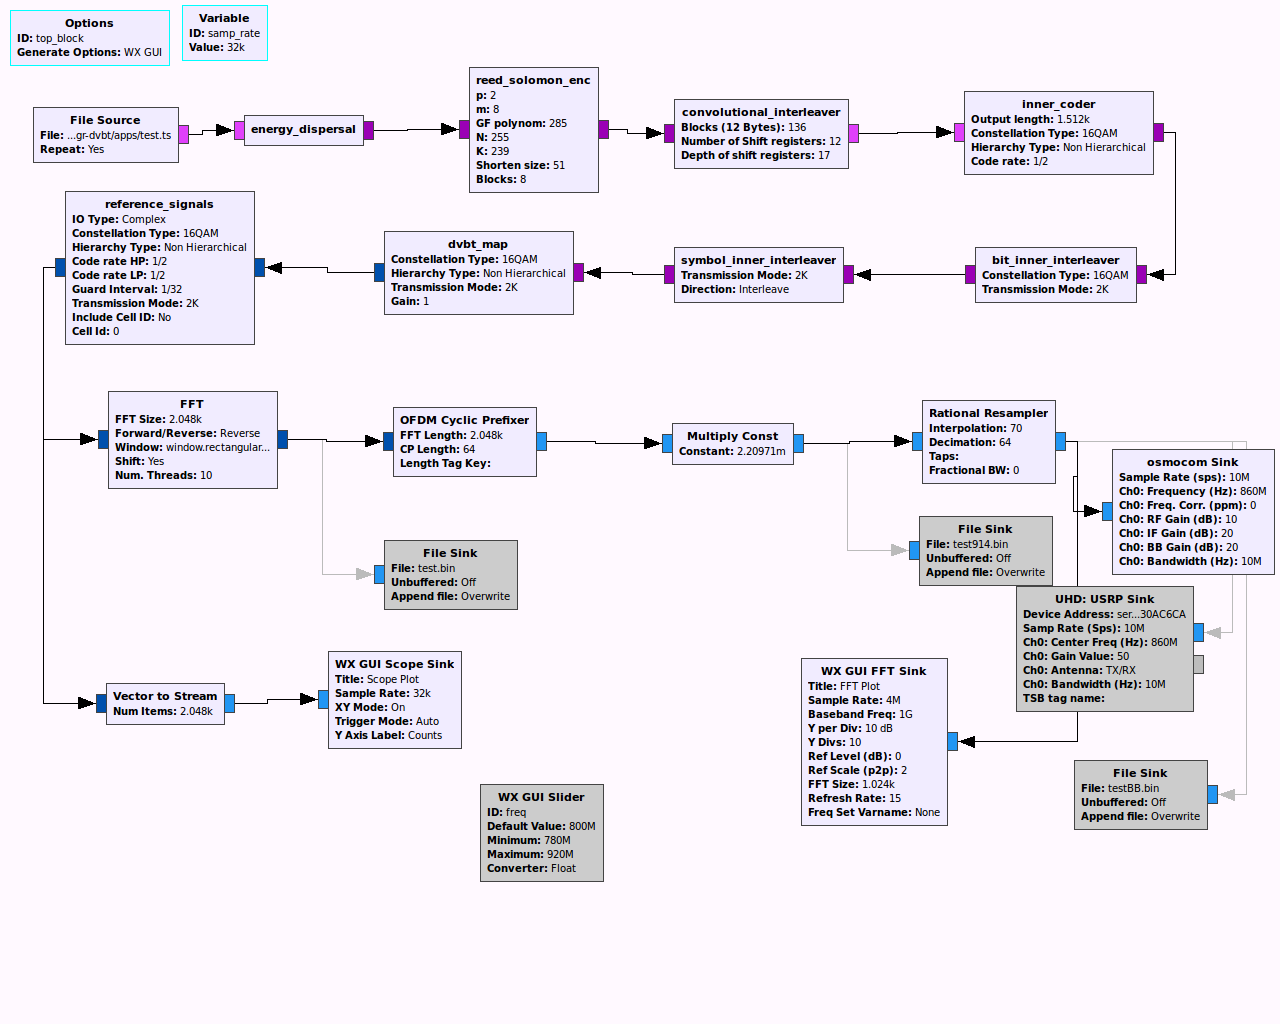
\includegraphics[height=13cm,angle=-90]{figures/dvbt_tx.png}
			\caption{GNU Radio DVB-T发射端}
			\label{fig:gnuradio_dvbt_tx}
		\end{figure}
		\begin{figure}[htb]
			\centering
			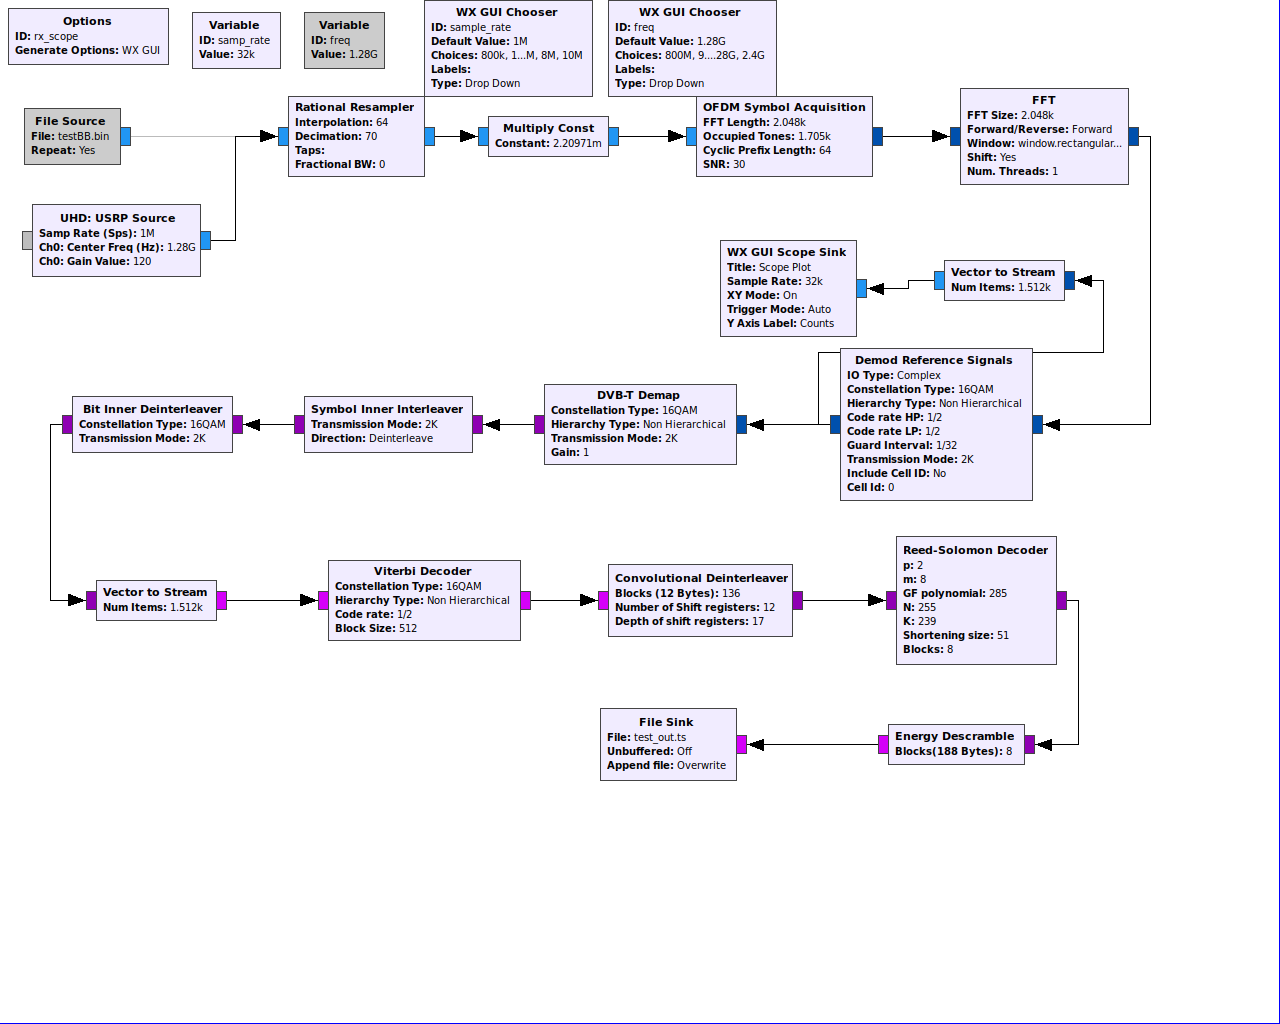
\includegraphics[height=13cm,angle=-90]{figures/dvbt_rx.png}
			\caption{GNU Radio DVB-T接收端}
			\label{fig:gnuradio_dvbt_rx}
		\end{figure}
	\section{设备连接}
		% TODO:图片标注
		\par 按图\ref{fig:devices}将设备连接,需要将USRP连接至USB3.0上,因为USB2.0的传输速率为8MS/s @ 16-bit I/Q,USB3.0的传输速率为61.44MS/s @ 16-bit I/Q\cite{USRP:SamplingRates}。
		\begin{figure}[htp]
			\centering
			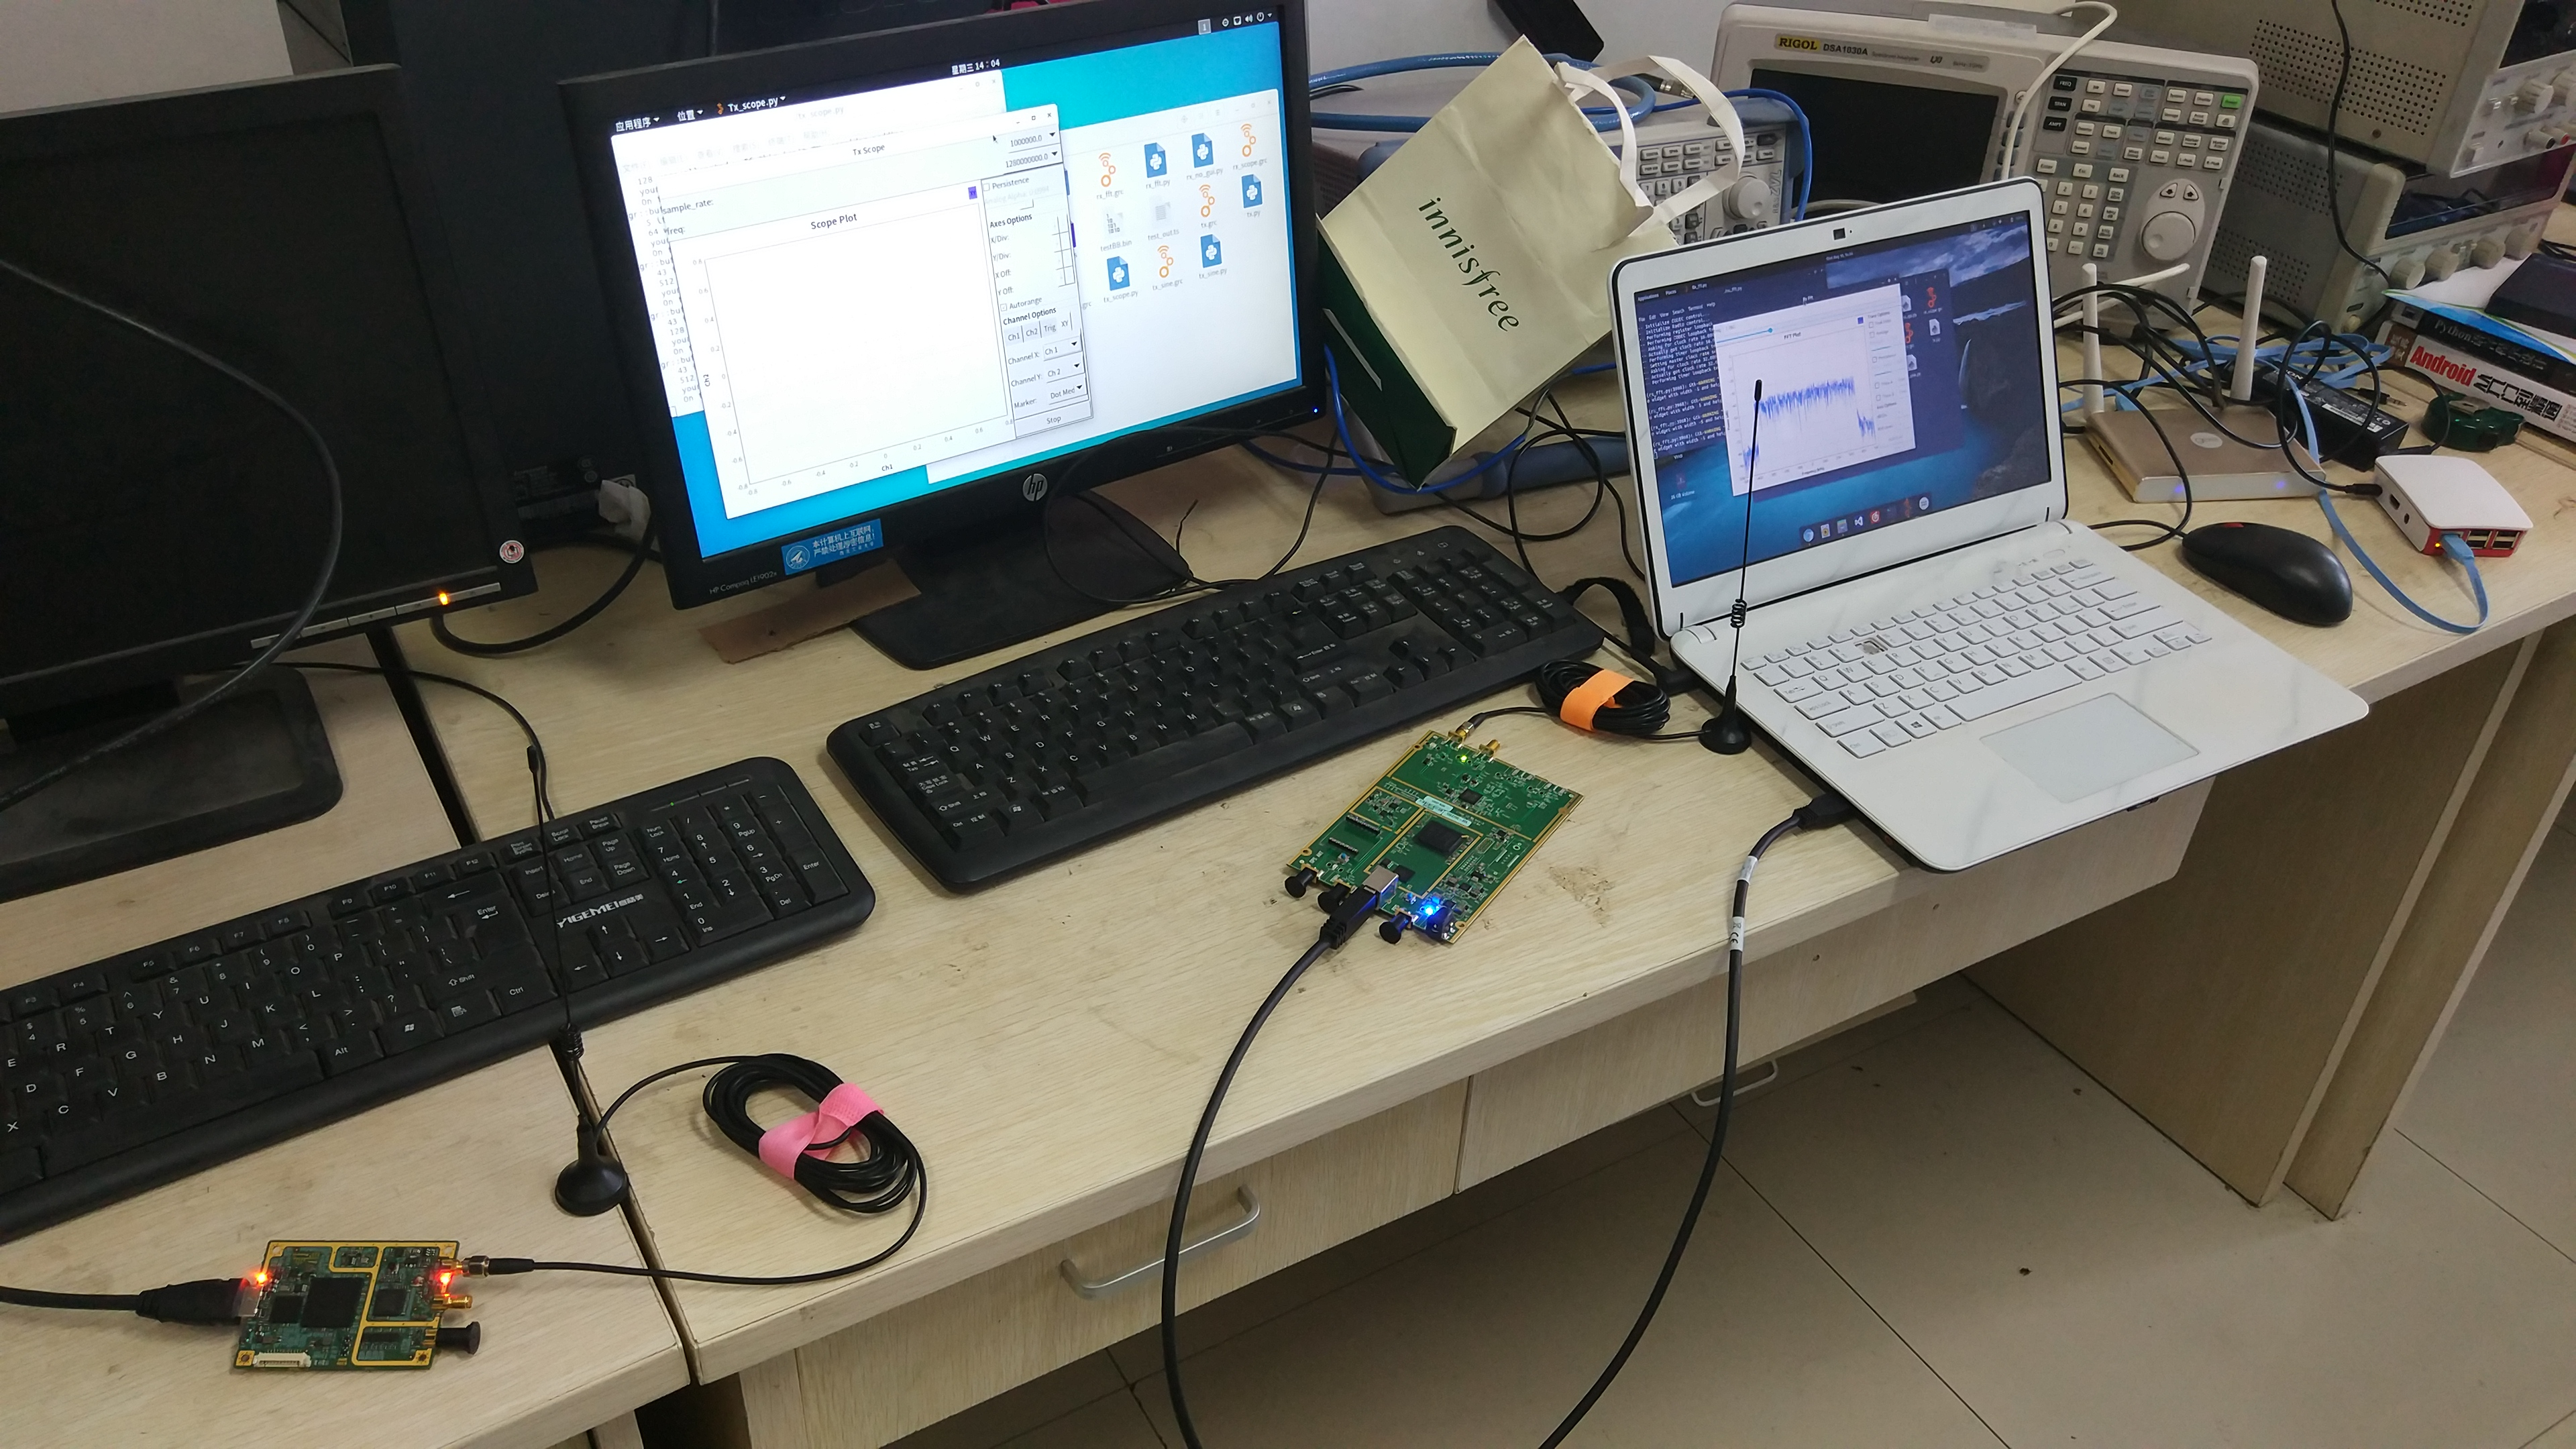
\includegraphics[width=13cm]{figures/devices.jpg}
			\caption{设备连接}
			\label{fig:devices}
		\end{figure}
	\section{运行程序}
		\par 点击GNU Radio中的运行(Run)按钮如图\ref{fig:dvbt_run},会在当前界面中直接运行该程序,直接运行可能会提示\lstinline[language=sh]{file not found}的错误,此时需要在\lstinline[language=sh]{file source}框图中指定文件的绝对位置,生成Python文件则只需要在同一目录下即可。
		\begin{figure}[htp]
			\centering
			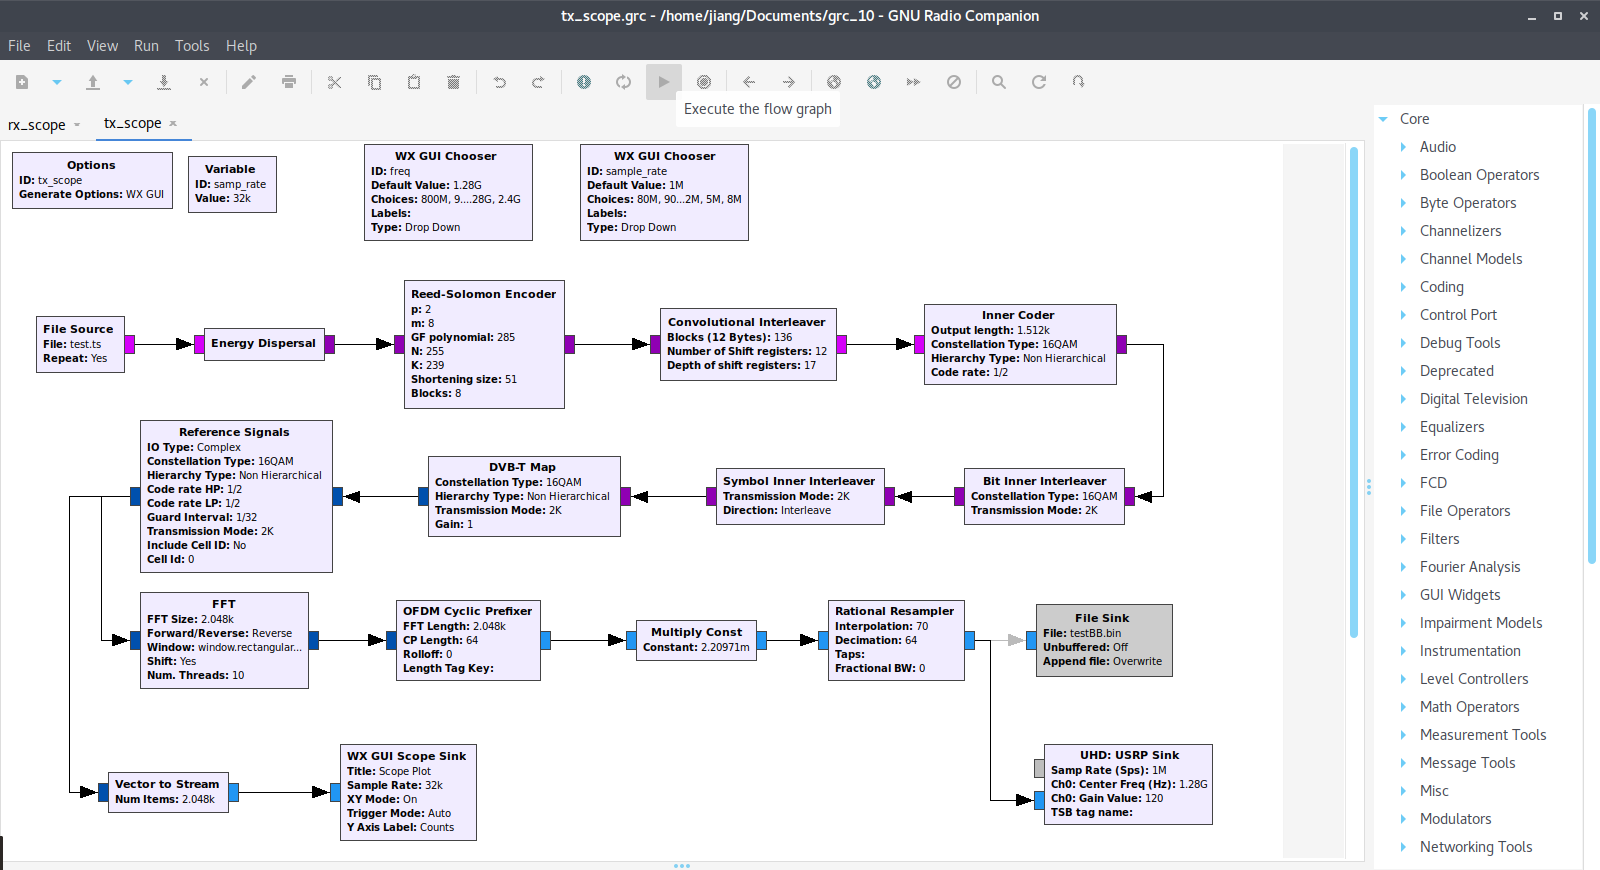
\includegraphics[width=13cm]{figures/dvbt_run.png}
			\caption{在当前界面中运行}
			\label{fig:dvbt_run}
		\end{figure}
		\par 点击GNU Radio上的生成(Generate)按钮如图\ref{fig:dvbt_generate},会成成一个于Options框图中ID相对应的Python文件(默认为\lstinline[language=sh]{top_block.py}),进入该文件所在目录,执行:
		\begin{figure}[htp]
			\centering
			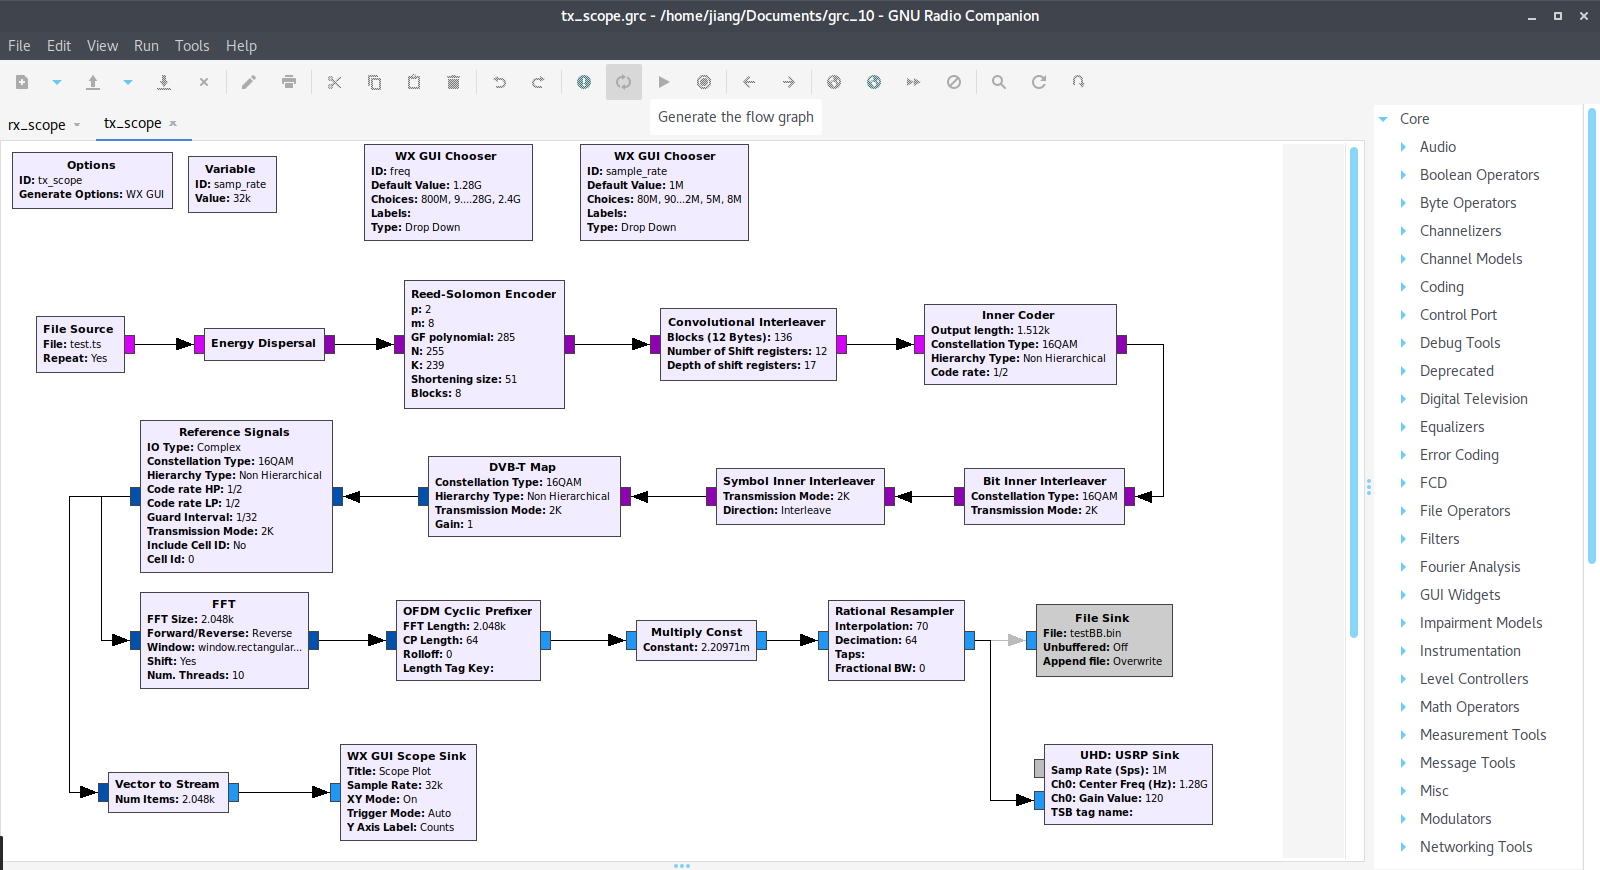
\includegraphics[width=13cm]{figures/dvbt_generate.png}
			\caption{生成Python文件}
			\label{fig:dvbt_generate}
		\end{figure}	
		\begin{lstlisting}[ language = sh ]
python top_block.py
		\end{lstlisting}
		\par 将其中的\lstinline[language=sh]{top_block.py}改为与之对应的文件名,如果出现\lstinline[language=sh]{no module named gnuradio}是因为当前的运行环境为Python3,则执行以下命令:
		\begin{lstlisting}[ language = sh ]
python2.7 top_block.py
		\end{lstlisting}
		\par 出现如图\ref{fig:dvbt_runtime},即表示正常运行。
		\begin{figure}[htp]
			\centering
			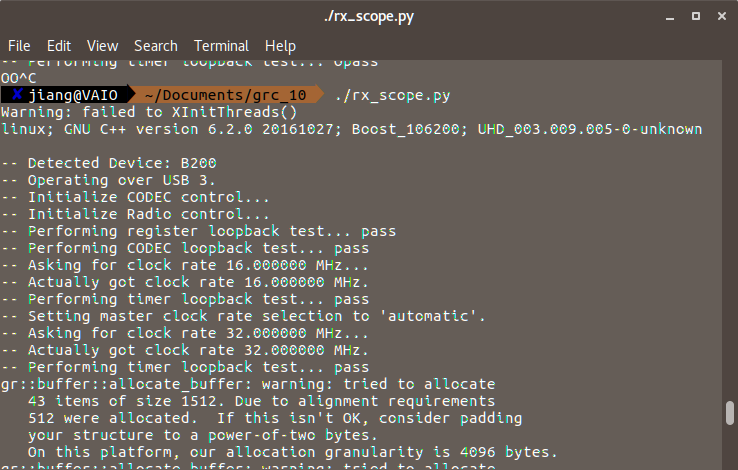
\includegraphics[width=13cm]{figures/dvbt_runtime.png}
			\caption{运行程序}
			\label{fig:dvbt_runtime}
		\end{figure}
		
				
